%!TEX root=../../autopilot.tex
\section{Data}
\label{sec:datamodel}

As of v0.5.0, Autopilot uses \href{https://pydantic-docs.helpmanual.io/}{pydantic} to create explicitly typed and schematized data models. Submodules include \texttt{data} abstract \texttt{modeling} tools that define base model types like \texttt{Table}s, \texttt{Group}s, and sets of \texttt{Attributes}. These base modeling classes are then built into a few core data models like subject \texttt{Biography} information, \texttt{Protocol} declaration, and the \texttt{Subject} data model itself that combines them. Modeling classes then have multiple \texttt{interfaces} that can be used to create equivalent objects in other formats, like pytables for hdf5 storage, pandas dataframes for analysis, or exported to Neurodata Without Borders.

For example, consider a simplified version of the \texttt{Biograpphy} model:


\begin{pythoncode*}{label = \texttt{\textbf{data - Biography}}}
from autopilot.data.modeling import Data, Attributes
from typing import Optional, Union

class Enclosure(Data):
    """Where does the subject live?"""
    box:  Optional[Union[str, int]] = Field(
        default=None, 
        description="The box this Subject lives in"
    )
    room: Optional[Union[str, int]] = Field(
        default=None, 
        description="The room number that the animal is housed in"
    )

class Biography(Attributes):
    """Biography of an Experimental Subject"""
    id:  str = Field(...
        description="The indentifying name of this subject."
    )
    dob: datetime = Field(... 
        description="The Subject's date of birth"
    )
    enclosure: Optional[Enclosure] = None

    @property
    def age(self) -> timedelta:
        """Difference between now and :attr:`.dob`"""
        return datetime.now() - self.dob
\end{pythoncode*}

A new subject could then be created with this biography like this, storing it in the HDF5 file and returning an exact copy when requested:

\begin{pythoncode*}{label = \texttt{\textbf{data - New Subject}}}
from autopilot.data import Subject

bio = Biography(
    id="my_subject",
    dob="2022-01-01T00:00:00",
    enclosure=Enclosure(box=100, room="Building 200")
)
sub = Subject.new(bio)
assert sub.info == bio
\end{pythoncode*}

The models are declared using a combination of python type hints\sidenote{Python \href{https://docs.python.org/3/library/typing.html}{type hints} are colon delimited annotations like this: \mintinline{python}{x:int = 1} that indicate the type (integer, string, etc.) of the variable. Though typically Python does not, Pydantic both validates that a type matches its hint and coerces it to the correct type if possible.} and \texttt{Field} objects that provide defaults and descriptions. Because these models can be recursive, as in the case of using the \texttt{Enclosure} model as a type within the \texttt{Biography} model, we can build expressive, flexible, but still strict representations of complex data. 

Out of the box, pydantic models can create explicit and interoperable \href{https://pydantic-docs.helpmanual.io/usage/schema/}{schemas} in \href{https://json-schema.org/draft/2020-12/json-schema-core.html}{JSON Schema} and \href{https://github.com/OAI/OpenAPI-Specification}{OpenAPI} formats, and Autopilot extends them with additional interfaces and representations. Autopilot can create a GUI form for filling in fields for models, for example, to create a new Subject or declare parameters for a task (Figure \ref{fig:modelform}). \texttt{Attribute} models that consist of scalar key-value pairs can be reliably stored and retrieved from metadata attribute sets in HDF5 groups, but Autopilot knows that \texttt{Table} models should be created as HDF5 tables as they will have multiple values for each field. An additional \texttt{Trial\_Data} class that inherits from \texttt{Table} can be exported to NWB trial data, and the \texttt{Subject.get\_trial\_data} method uses the model to load trial data and convert it to a correctly typed pandas\citep{mckinneyPandasFoundationalPython2011} DataFrame.

\begin{marginfigure}
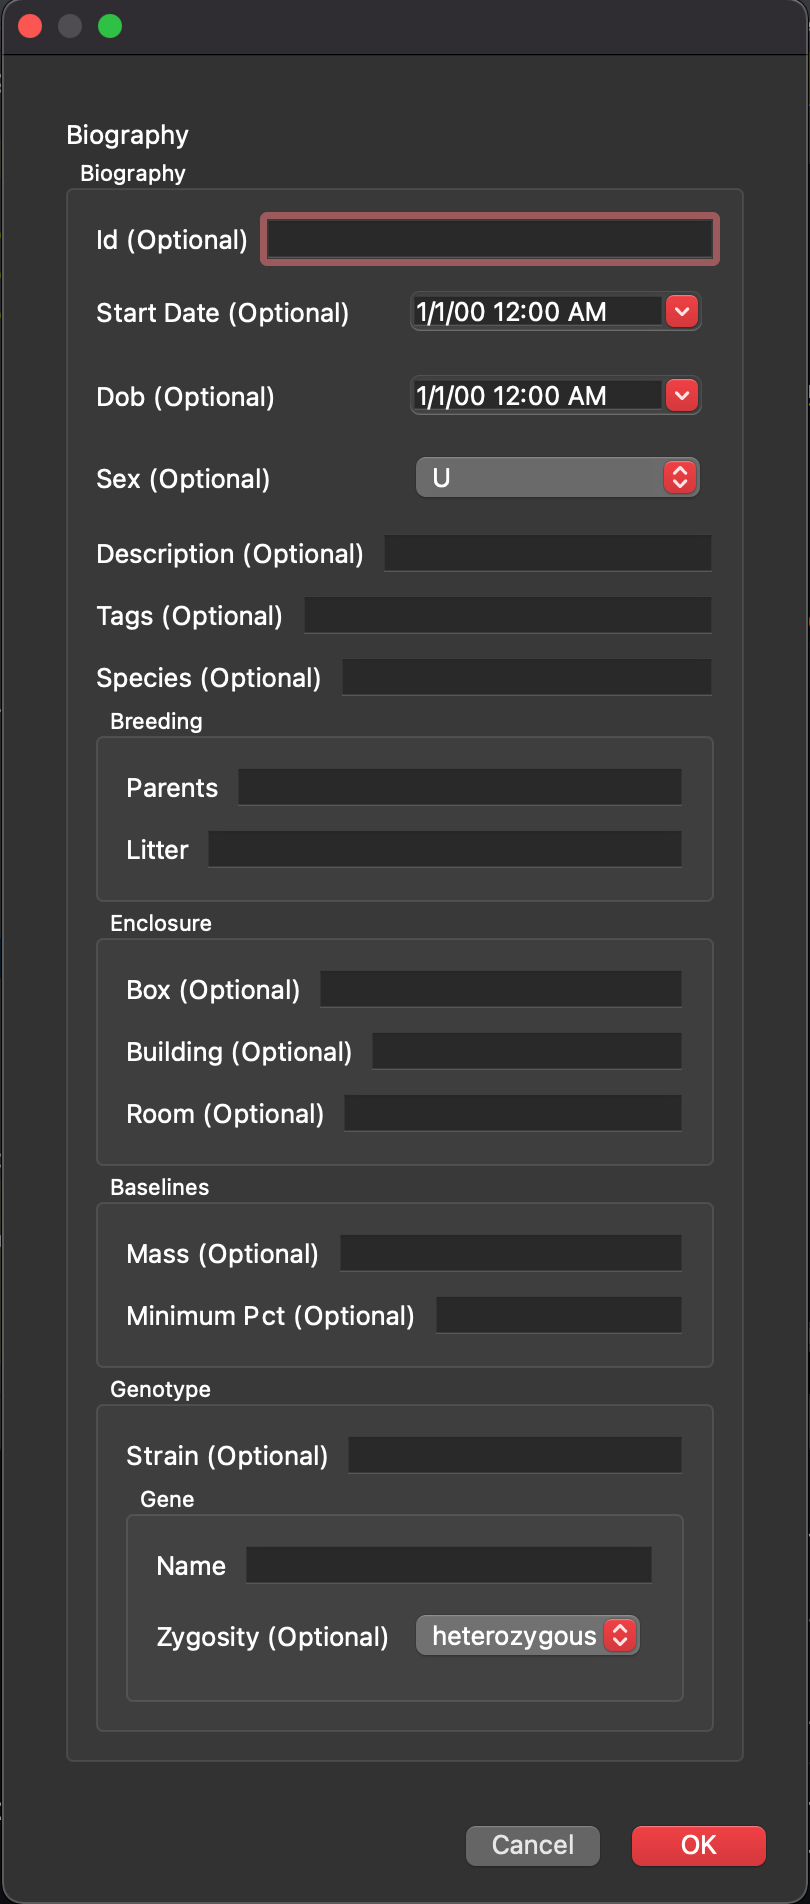
\includegraphics[width=\linewidth]{figures/model_form.png}
\label{fig:modelform}
\caption{An Autopilot Data model can automatically generate a GUI form to fill in its properties, in this example to define a new experimental Subject's biography.}
\end{marginfigure}

Though the data modeling system is new\sidenote{Released as an alpha version at the time of writing}, we have laid the groundwork for Autopilot's plugin system to allow researchers to declare custom schema for all data produced by Autopilot, and to preserve both interoperability and reproducibility by combining them with datasets potentially produced by multiple incompatible tools (see \ref{sec:future}).



